\chapter{Livello di rete: control plane}
\section{Introduzione}
Le tabelle di forwarding e di flow sono computate e mantenute secondo due approcci:
\begin{itemize}
\item Per-router control: un algoritmo di routing viene eseguito su ogni router della rete in cui sono contenute funzioni di routing e forwarding. Ogni 
router possiede una componente di routing che comunica con quella degli altri router per computare i valori della tabella di forwarding. I protocolli di 
OSPF e BGP sono basati su questo approccio.
\item Logically centralized control: un controller centralizzato computa e distribuisce le tabelle di forwarding, permette di implementare numerose funzioni
attraverso una flow table. Il controller interagisce con ogni agente di controllo in ogni router attraverso un protocollo ben definito e non interagisce con
altri CA. 
\end{itemize}
\section{Algoritmi di routing}
Lo scopo di questi algoritmi \`e quello di determinare i cammini ottimi o routes da mittente e destinatario attraverso la rete di router. Un grafo \`e 
utilizzato per formulare questo problema in cui i nodi rappresentano router e gli archi i collegamenti tra di essi. Ogni arco ha un valore che rappresenta
il suo costo che riflette la lunghezza fisica del link, la sua velocit\`a di trasmissione e il costo economico. Per un arco $(x, y)$ si indica il costo 
attraverso $c(x, y)$, se l'arco non appartiene al grafo $c(x, y)=+\infty$. L'obiettivo naturale per questo algoritmo \`e pertanto quello di trovare il 
cammino meno costoso tra due nodi. 
\begin{itemize}
\item Un algoritmo di routing centralizzato computa il cammino meno costoso utilizzando una conoscenza completa della rete, ovvero prende come input il 
grafo contenente tutti i nodi e tutti i link. Questi algoritmi sono detti algoritmi link-state (LS).
\item Un algoritmo di routing decentralizzato il calcolo del cammino meno costoso \`e effettuata in maniera distribuita dai router. Nessun nodo possiede 
conoscenza completa della rete, ma conosce unicamente i costi dei link a lui direttamente attaccati. Successivamente attraverso un processo iterativo di 
calcoli e di scambio di informazioni con altri nodi vicini il nodo calcola gradualmente il cammino meno costoso per un insieme di destinazioni. 
\end{itemize}
Gli algoritmi di routing si possono classificare anche in base al fatto che siano statici (dove routes cambiano raramente) o dinamici (dove routes cambiano
dinamicamente in maniera responsiva in base a cambi di topologia o di costo dei link: si ottengono per esempio eseguendoli periodicamente. Un ulteriore 
metodo di classificazione si basa sul fatto se gli algoritmi sono load-sensitive o no in cui i costi dei link variano dinamicamente in base al livello di 
congestione della rete. 
\subsection{L'algoritmo di link state routing}
In modo da ottenere la topologia di rete e i costi dei link ogni nodo fa un broadcast link-state su tutti gli altri nodi della rete con ogni pacchetto 
contenente identit\`a e costo di ogni link del nodo. In questo modo tutti i nodi hanno una visione completa e globale della rete. L'algoritmo link-state di
routing \`e conosciuto come algoritmo di Dijkstra: questo algoritmo computa il cammino di costo minore da un nodo a tutti gli altri nodi nel pacchetto. 
Questo algoritmo ha la propriet\`a che alla fine della k-esima iterazione sono conosciuti i cammini minimi per k nodi, Si definisca $D(v)$ come il costo 
del cammino ottimo dal nodo di origine $u$ fino al nodo di destinazione $v$ di questa iterazione, $p(v)$ come il nodo genitore in questa esplorazione. $N'$
come il sottoinsieme dei nodi tali per cui il cammino ottimo \`e stato trovato. L'algoritmo consiste di una fase di inizializzazione e di un loop eseguito
per ogni nodo del grafo. 
\begin{figure}[h]
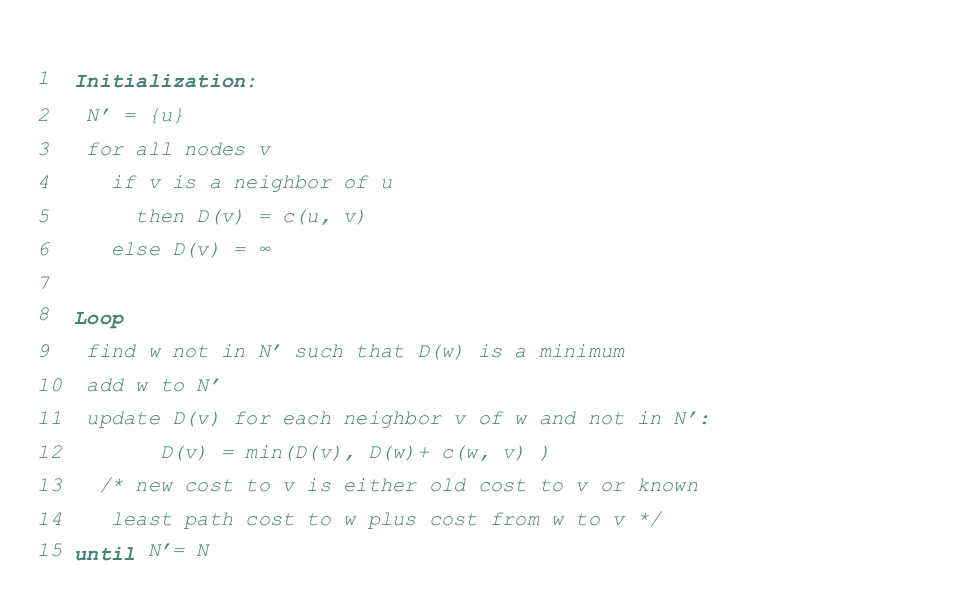
\includegraphics[width=\textwidth]{AlgoritmoDijkstra.png}
\caption{Algoritmo di Dijkstra}
\end{figure}
Quando l'algoritmo LS termina si ha per ogni nodo il suo predecessore e il cammino ottimo dal nodo di origine. La tabella di forwarding \`e costruita 
salvando per ogni destinazione il prossimo hop nel cammino ottimo. Questo algoritmo ha complessit\`a $O(n^2)$. 
\subsection{L'algoritmo di distance vector routing}
L'algoritmo di distance vector \`e iterativo, asincrono e distribuito. \`E distribuito nel senso che ogni nodo riceve informazioni da uno o pi\`u dei suoi
diretti vicini, svolge un calcolo e ritorna i dati ai vicini. \`E asincrono in quanto non richiede che i vicini operino in lockstep l'uno con l'altro ed \`e
self-terminating. Si consideri $d_x(y)$ il cammino ottimo da $x$ a $y$ e $v$ ogni vicino di $x$, allora secondo l'equazione di Bellman-Ford $d_x(y)=\min_v
\{c(x, v)+d_v(y)\}$. La soluzione a questa equazione d\`a le entries da mettere nella tabella di forwarding: si consideri $v*$ ogni nodo vicino che risolve
l'equazione allora la tabella deve indicarlo come prossimo hop per raggiungere infine $y$. Per trovare tali valori ogni nodo $x$ comincia con $D_x(y)$, una
stima del costo del cammino ottimo da s\`e stesso a qualsiasi nodo in $N$. Sia $D_x=\{D_x(y):y\in N\}$ il vettore delle distanze del nodo $x$, ovvero il
vettore della stima dei costi del cammino ottimo. Con l'algoritmo DV l'algoritmo di routing mantiene le seguenti informazioni:
\begin{itemize}
\item Per ogni vicino $v$, il costo $c(x, v)$.
\item Il vettore delle distanze di $x$, ovvero $D_x$.
\item Il vettore delle distanze di ogni suo vicino, ovvero $D_v$ per ogni vicino $v$.
\end{itemize}
Nell'algoritmo distribuito e asincrono ogni tanto ogni nodo manda una copia del suo vettore delle distanze ai suoi vicini che lo salvano e lo utilizzano
per aggiornare il proprio vettore delle distanze seguendo l'equazione di Bellman-Ford: $D_x(y)=\min_v\{c(x, v)+D_v(y)\}$ per ogni nodo $y$ in $N$. Se il 
vettore delle distanze viene modificato nel passo di aggiornamento $x$ invia una copia ad ogni vicino. Se tutti i nodi continuano a scambiarsi i vettori 
delle distanze in maniera asincrona ogni stima $D_x(y)$ converge a $d_x(y)$ il costo ottimo reale. 
\begin{figure}[h]
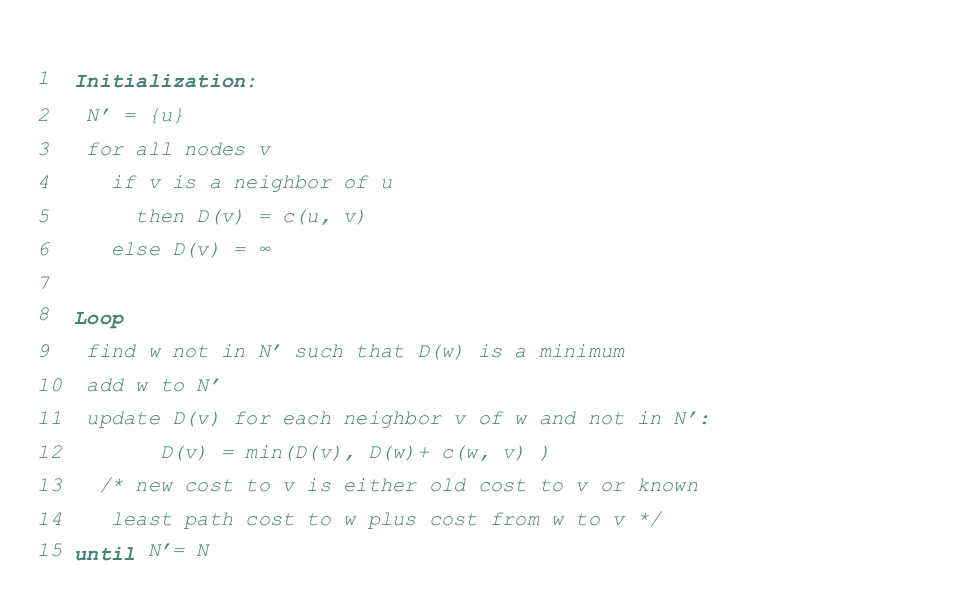
\includegraphics[width=\textwidth]{AlgoritmoDijkstra.png}
\caption{Algoritmo Distance Vector}
\end{figure}
Quello che interessa non \`e la lunghezza del cammino minimo, ma il vicino $v*$ obiettivo del prossimo hop, pertanto nelle righe 13-14 del codice si
prende il vicino che ha il valore minimo e lo si inserisce nella tabella. 
\subsubsection{Cambio di costo dei link e loro fallimento}
Quando un nodo che esegue l'algoritmo DV percepisce un cambio di costo in un link aggiorna il suo vettore delle distanze e se avviene un cambio nei percorsi
ottimi informa i suoi vicini. Questi aggiornamenti a causa della loro localit\`a possono causare dei routing loop che possono essere molto difficili da
risolvere, anche se poi verranno risolti. Questi problemi sono chiamati count-to-infinity problem. 
\subsubsection{Aggiungere poisoned revers}
Lo scenario appena descritto pu\`o essere evitato aggiungendo una poisoned reverse: se un nodo instrada il pacchetto verso quello che gliel'ha inviato gli 
mente inviandogli che la sua distanza dalla destinazione finale \`e $\infty$ fino a che $z$ continuer\`a a fare routing verso la destinazione da tale nodo.
Credendo che non ci sia cammino il primo mittente cambier\`a cammino. Questa tecnica risolve il count-to-infinity problem unicamente se il loop accade su 
nodi vicini. 
\subsection{Confronto tra LS e DV}
Si indichi con $N$ il numero di nodi e con $E$ il numero di archi:
\begin{itemize}
\item Complessit\`a dei messaggi: essendo che LS richiede che ogni nodo conosca il costo di ogni link nella rete vengono richiesti $O(|V|+|E|)$ messaggi per router e 
il cambio di costo di un link deve essere comunicato a tutti i nodi. DV richiede uno scambio di messaggi unicamente tra vicini ad ogni iterazione ma il costo
di convergenza dipende da molti cammini. Il cambio di costo di un link causa una propagazione di messaggi unicamente se cambia un cammino ottimo.
\item Velocit\`a di convergenza: LS \`e un algoritmo in $O(|N|^2)$ messaggi che richiede $O(|V|+|E|)$ messaggi. L'algoritmo DV pu\`o convergere lentamente
e incontrare routing loop e il count-to-infinity problem.
\item Robustezza: i calcoli dei cammini sono separati in LS offrendo della robustezza mentre in DV dipendono dai calcoli dei vicini e pertanto se c'\`e un
malfunzionamento questo pu\`o diffondersi in tutta la rete.
\end{itemize}
\section{Intra-AS routing nell'internet: OSPF}
Il modello che considera l'internet come un omogeneo insieme di router che eseguono tutti lo stesso algoritmo \`e semplicistico per due ragioni:
\begin{itemize}
\item Scala: con la crescita del numero di router l'overhead necessaria a calcolare, comunicare e salvare le informazioni di routing diventa proibitiva. 
\item Autonomia amministrativa: l'internet \`e una rete di ISPs che possiedono la propria rete di routers. Queste ISP desiderano operare in maniera pi\`u
autonoma possibile e amministrare la propria rete secondo il loro desiderio ma essere capaci di connettere la loro rete con le altre.
\end{itemize}
Entrambi questi problemi possono essere risolti organizzando i router in sistemi autonomi (ASs) consistenti di insiemi di router sotto lo stesso controllo
amministrativo, identificato globalmente dal suo autonomous system number (ASN), assegnati anche loro da ICANN. Router nello stesso AS eseguono lo stesso 
algoritmo di routing e possiedono informazioni gli uni degli altri. Questo algoritmo di routing \`e detto intra-autonomous system routing protocol. 
\subsection{Open shortest path first (OSPF)}
Il routing OSPF e il suo simile IS-IS sono largamente utilizzati per le operazioni di routing per le intra-AS dell'internet. La parola Open indica che il 
protocollo \`e pubblicamente disponibile. Questo protocollo usa flooding di informazioni di link-state e un algoritmo di cammino 
ottimo di Dijkstra. Ogni router costruisce una mappa topologica completa dell'intero sistema autonomo, ogni router successivamente esegue Dijkstra per 
determinare l'albero di cammino minimo per ogni sottorete con s\`e stesso come radice (i costi di link sono configurati dall'amministratore di rete). Un router
fa un broadcast delle sue informazioni di link-state a tutti gli altri router ogni volta c'\`e un cambio in un link-state e periodicamente (almeno ogni 30
minuti). Questi messaggi sono trasportati direttamente da IP con un protocollo di livello pi\`u alto per OSPF che controlla se i link sono funzionanti. 
Alcuni dei vantaggi di OSPF sono:
\begin{itemize}
\item Sicurezza: scambi tra router OSPF possono essere autenticati: solo trusted router possono partecipare nelle tabelle. Si pu\`o utilizzare una password
in plaintext o MD5.
\item Cammini ottimi multipli: quando esistono multipli cammini ottimi tutti possono essere utilizzati. 
\item Supporto integrato per unicast e multicast broadcasting: MOSPF usa il link database OSPF e aggiunge un nuovo tipo di avvertimento link state al 
meccanismo di broadcast.
\item Supporto per gerarchie all'interno di un singolo AS: L'AS viene separato in aree comunicanti attraverso area border router. Un'area \`e designata come
backbone per fare routing tra le varie aree contiene tutti i router area border e anche altri. 
\end{itemize}
\section{Routing tra ISPs: BGP}
Per fare routing tra host in diverse AS si rende necessario un protocollo di inter-autonomous system routing. Tutte le AS comunicanti devono eseguire lo 
stesso protocollo chiamato il Border Gateway protocol BGP. \`E un protocollo asincrono e decentralizzato con un algoritmo di routing DV. 
\subsection{Routing BGP}
Se la destinazione di un pacchetto \`e esterna all'AS il pacchetto viene instradato verso prefissi CIDRized, con ognuno di essi rappresentanti una subnet o
un insieme di subnet. Pertanto un entry della tabella di forwarding avr\`a la forma $(x, I)$, con $x$ il prefisso e $I$ il numero di interfaccia di una 
delle interfacce del router. BGP mette a disposizione ad ogni router modi per:
\begin{itemize}
\item Ottenere informazioni di raggiungibilit\`a di prefissi da altri AS: permette ad ogni subnet di pubblicizzare la propria esistenza all'intero internet.
\item Determinare il cammino migliore per i prefissi.
\end{itemize}
\subsection{Pubblicizzare le informazioni di BGP route}
In un AS si distingue tra gateway router e router interni: i primi sono i router dell'AS che si connettono direttamente con router di altre AS. Per 
pubblicizzare la raggiungibilit\`a di un prefisso ogni AS manda un messaggio BGP agli AS vicini, che lo mandano a loro volta ai loro AS vicini indicando 
s\`e stessi come cammino intermedio. In BGP paia di router si scambiano informazioni attraverso una connessione TCP semi-permanente sulla porta 179. Ognuna
di queste in combinazione con il messaggi inviati \`e chiamata una connessione BGP. Una connessione BGP che attraversa pi\`u AS \`e detta esterna, 
altrimenti interna. Tipicamente si trova un eBGP per ogni link che connette due AS e un iBGP per ogni coppia di router all'interno dell'AS. I messaggi di 
raggiungibilit\`a sono pertanto propagati da una eBGP, successivamente distribuiti in tutta l'AS attraverso iBGP e poi ancora ad altre AS attraverso eBGP.
\subsection{Determinare il cammino ottimo}
Quando una connessione BGP pubblicizza un prefisso include ad esso vari attributi BGP formando una route. Due di questi attributi sono AS-PATH e NEXT-HOP.
Il primo contiene la lista di AS attraverso cui il messaggio di pubblicizzazione \`e passato, affinch\`e venga generato quando un prefisso \`e passato
ad un AS questo aggiunge ad esso il proprio ASN nella lista esistente in AS-PATH. Viene utilizzato anche per evitare loop di pubblicizzazione. L'attributo 
NEXT-HOP mette a disposizione il link tra i protocolli intra e inter AS e contiene l'indirizzo IP dell'interfaccia router che comincia l'AS-PATH.
\subsubsection{Hot potato routing}
In questo tipo di routing il cammino scelto \`e il cammino ottimo al router NEXT-HOP che comincia tale cammino. L'algoritmo pertanto opera in questa 
maniera:
\begin{itemize}
\item Apprende dal protocollo AS che una sottorete \`e raggiungibile da diversi gateways.
\item Usa il protocollo intra-AS per determinare il costo minimo a ciascuno di questi gateways.
\item Sceglie il gateway con il costo minore.
\item Determina dalla tabella di forwarding l'interfaccia che porta al gateway, inserisce $(prefisso, I)$ nella tabella. 
\end{itemize}
\subsubsection{Algoritmo di route-selection}
Per ogni dato prefisso di destinazione l'input di questo algoritmo \`e l'insieme di tutti i cammini verso quel prefisso che sono conosciute e accettate, se 
sono pi\`u di una invoca le seguenti regole di eliminazione fino a che ne rimane una sola:
\begin{itemize}
\item Un route \`e assegnato un valore di local preference come attributo. Le routes con il maggior valore di local preference sono selezionate.
\item Dalle routes rimanenti sono selezionate quelle con l'AS-PATH minore. 
\item Si seleziona dalle routes rimanenti utilizzando hot potato.
\item Se rimangono ancora pi\`u routes vengono utilizzati i BGP identifiers. 
\end{itemize}
\subsection{IP anycast}
BGP \`e utilizzato per implementare il servizio di IP anycast usato comunemente dai DNS. Viene utilizzato in quanto si \`e interessati a duplicare contenuti
in diversi server dispersi geograficamente e far accedere ogni utente al server pi\`u vicino. Durante la fase di configurazione dell'anycast una compagnia
assegna lo stesso indirizzo IP ai suoi server e usa BGP per pubblicizzare ognuno di questi. Quando un router riceve questi multipli li tratta come se 
mettessero a disposizione diverse routes per la stessa destinazione. 
\subsection{Politica di routing}
Il cambio della local preference \`e utilizzato per determinare delle zone protette dove non si devono svolgere operazioni di routing o per scegliere altri
cammini in modo da rispettare politiche dell'ISP. 
\section{The SDN control plane}
Si possono identificare quattro caratteristiche fondamentali di un'architettura SDN:
\begin{itemize}
\item Flow-based forwarding.
\item Separazione tra il data plane e il control plane con il primo hardware e il secondo software.
\item Funzioni di controllo di rete esterne agli switch data plane.
\item Rete programmabile. 
\end{itemize}
\subsection{Il control plane dell'SDN, controller e applicazioni di controllo di rete}
Il control plane dell'SDN si divide in due componenti principali: un controller SDN e le applicazioni di controllo di rete. Le funzionalit\`a di un 
controller di possono dividere in tre categorie:
\begin{itemize}
\item Un livello di comunicazione tra il controller e i dispositivi connessi alla rete attraverso un protocollo conosciuto come l'interfaccia "southbound"
del controller.
\item Un livello di gestione dello stato per tutta la rete in quanto decisioni prese dal controller richiedono informazioni riguardo tutta la rete. 
\item Un interfaccia verso le applicazioni di controllo di rete detta anche interfaccia "northbound" in modo di permettere a funzioni di leggere e scrivere
all'interno del livello di gestione di stato della rete. 
\end{itemize}
Il controller \`e logicamente centralizzato ma in realt\`a \`e costituito da diversi server con database e algoritmi distribuiti. 
\subsection{Il protocollo OpenFlow}
Il protocollo OpenFlow opera tra il controller e uno switch controllato da SDN, opera attraverso TCP con porta 6653. Tra i messaggi inviati dal controller
allo switch figurano:
\begin{itemize}
\item Configurazione: per fare query e settare i parametri di configurazione di uno switch.
\item Modifica di stato: per aggiungere o eliminare entries nelle tabelle di flow o per cambiare propriet\`a di porte.
\item Lettura di stato: utilizzato per collezionare statistiche e contatori dalle porte e tabelle dello switch. 
\item Invio di pacchetto: utilizzato per mandare uno specifico pacchetto ad una porta specifica allo switch il messaggio contiene il pacchetto che deve 
essere mandato come suo payload.
\end{itemize}
Tra i messaggi inviati dallo switch al controller figurano:
\begin{itemize}
\item Flow rimosso: informa il controller che un entry nella tabella di flow \`e stata rimossa. 
\item Status di porta: informa il controller in un cambio di status in una porta.
\item Packet-in: manda al controller il pacchetto senza entry nella tabella di flow. 
\end{itemize}
\section{ICMP il protocollo di internet control message}
Il protocollo di internet control message \`e utilizzato da host e router per comunicare informazioni di livello di rete tra di loro. L'utilizzo pi\`u comune \`e il report degli errori.  Architetturalmente si trova appena
sopra IP in quanto messaggi ICMP sono spostati come payload di IP. Quando un host riceve un datagramma IP con ICMP specificato come il protocollo di livello superiore (con numero 1) fa demultiplexing a 
ICMP. I messaggi ICMP hanno un tipo e in campo di codice e contengono l'header e i primi 8 bytes del datagramma IP che ha causato la generazione del messaggio in modo che il mittente pu\`o determinare
quale datagramma ha generato l'errore.  
\begin{figure}[h]
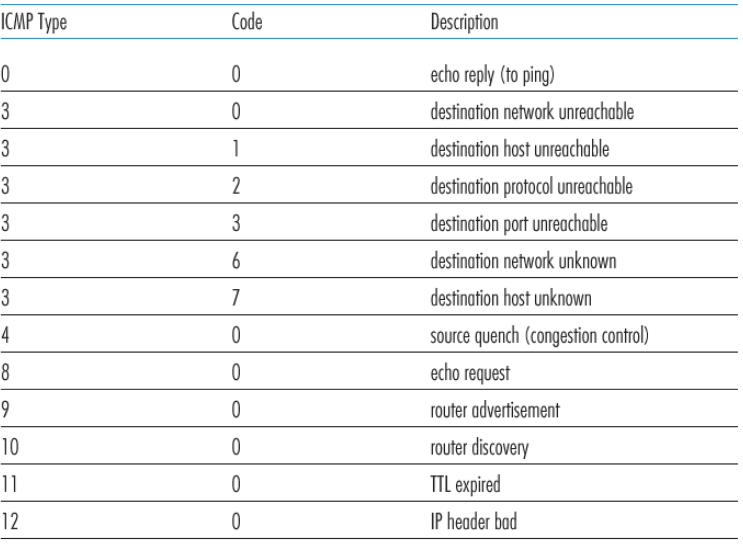
\includegraphics[width=\textwidth]{ICMPValues.png}
\caption{Tipi di messaggio ICMP}
\end{figure}
Traceroute utilizza questi messaggi generando pacchetti UDP con TLL incrementale su una con range tra 33434 e 33534 fino a che arriva a ricevere un messaggio ICMP di tipo 3 con codice 3.
\section{Gestione della rete e SNMP}
La gestione della rete include distribuzione, integrazione e coordinazione dell'hardware, software e elementi umani per monitorare, testare, sondare, configurare, analizzare, valutare e controllare la rete e le
risorse elementari in tempo reale, con prestazioni operazionali e servizio di qualit\`a ad un costo ragionevole. 
\subsection{Il framework per la gestione della rete}
Le componenti chiave della gestione di rete sono:
\begin{itemize}
\item Il managing server, un'applicazione con un umano nel ciclo che viene eseguita nel centro delle operazioni di rete (NOC) che controlla la collezione, processing, analisi e visione di attivit\`a della gestione di 
rete. \`E qui che le azioni sono iniziate per controllare il comportamento della rete.
\item Un managing device, un equipaggiamento di rete che si trova sulla rete gestita che gestisce dei managed objects che sono strumenti hardware e la configurazione dei loro parametri.
\item Un management information base (MIB) che raccoglie le informazioni di ogni managed object e le mette a disposizione del managing server. Questi parametri sono specificati in SMI (structure of 
management information). 
\item Il network management agent \`e il processo che comunica con il managing server.
\item Il network management protocol che viene eseguito tra il managing server e i managed device in modo da permettere la comunicazione e le query tra i due. 
\end{itemize}
\subsection{Il simple network management protocol (SNMP)}
SNMP \`e un protocollo di livello applicativo utilizzato per trasportare controllo di gestione della rete e informazioni  tra un managing server e un agente che esegue al suo posto. L'utilizzo pi\`u comune \`e in
modalit\`a request-response in cui un managing server SNMP invia una richiesta ad un agente SNMP che la riceve, svolge qualche azione e invia una risposta alla richiesta. Le richieste sono utilizzate per query o 
per modificare oggetti MIB. Viene anche utilizzato per mandare trap message al managing server per notificarlo di situazioni eccezionali. Vengono definiti sette tipi di messaggi detti protocol data units (PDUs).
\begin{itemize}
\item I messaggi \emph{GetRequest, GetNextRequest} e \emph{GetBulkRequest} sono inviate dal managing server per richiedere valori di uno o pi\`u oggetti MIB al managed device dell'agente. Gli oggetti 
richiesti sono specificati nella porzione di variable binding. L'agente risponde con una PDU di risposta che contiene gli identificatori degli oggetti e i valori associati.
\item Il PDU \emph{SetRequest} \`e utilizzato dal managing server per settare i valori di uno o pi\`u oggetti MIB in un managed device. UN agente risponde con un PDU di risposta con lo status di errore
noError per confermare che il valore \`e stato settato. 
\item Il PDU \emph{InformationRequest} \`e utilizzato dal managing server per notificare un altro managing server di informazioni MIB che sono remote al server destinatario.
\item Il PDI \emph{Response} \`e tipicamente mandato da un managed device in risposta ad un request message ritornando le informazioni richieste.
\item Il tipo finale \`e il trap message, sono generati asincronamente, ovvero non sono generati in risposta a richieste ma in risposta a eventi per i quali il server richiede notifica. 
\end{itemize}
Sono tipicamente trasmessi attraverso UDP.
\begin{figure}[h]
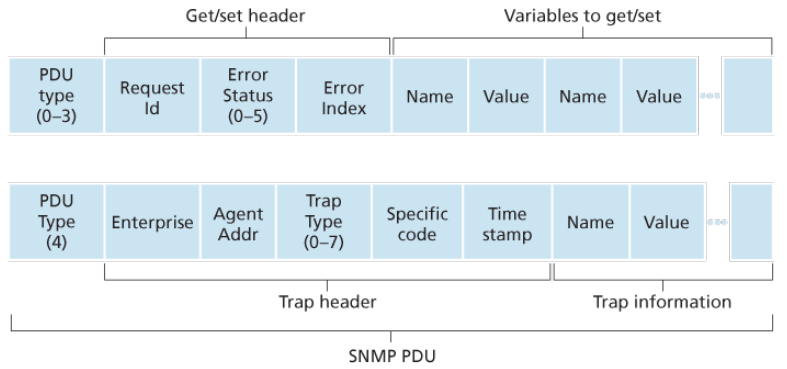
\includegraphics[width=\textwidth]{SNMPPDUFormato.png}
\caption{Formato di un PDU SNMP}
\end{figure}